% !TEX program = pdflatex
\documentclass[letterpaper, 10 pt, conference]{ieeeconf}
\usepackage{graphicx}

\overrideIEEEmargins

\usepackage[utf8]{inputenc}
\usepackage[T1]{fontenc}
\usepackage{graphics}
\usepackage{amsmath}
\usepackage{amssymb}
\usepackage{booktabs}
\usepackage{multirow}

\setlength{\textfloatsep}{5pt plus 1pt minus 1pt}
\setlength{\floatsep}{4pt plus 1pt minus 1pt}
\setlength{\intextsep}{4pt plus 1pt minus 1pt}

\title{\LARGE \bf
Clasificación de Estudios MRI Cerebrales mediante Redes Neuronales Convolucionales para la Detección de Tipos de Tumor
}

\author{Otto Wilmer Castillo Santacruz, Edgar Andrés Pérez Mora y Silvio Yopasa Romero\\
\textit{Maestría en Inteligencia Artificial (MAIA), Universidad de los Andes, Bogotá, Colombia}\\
{\tt\small \{o.castillos, ea.perezm1, s.yopasa\}@uniandes.edu.co}
}

\begin{document}

\maketitle
\thispagestyle{empty}
\pagestyle{empty}

%%%%%%%%%%%%%%%%%%%%%%%%%%%%%%%%%%%%%%%%%%%%%%%%%%%%%%%%%%%%%%%%%%%%%%%%%%%%%%%%
\section{Introducción}

La resonancia magnética cerebral (\textit{Magnetic Resonance Imaging}, MRI) es la modalidad de imagen de referencia para la detección no invasiva, caracterización morfológica y planificación terapéutica de neoplasias intracraneales \cite{c1}. En la práctica clínica, la interpretación visual de múltiples cortes anatómicos exige alta especialización radiológica y está sujeta a variabilidad interobservador. Las redes neuronales convolucionales (CNN) permiten extraer representaciones jerárquicas directamente de los niveles de intensidad en cortes bidimensionales (2D), apoyando el diagnóstico asistido por computador \cite{c2}.

El problema abordado consiste en la clasificación supervisada multiclase de cortes 2D de MRI cerebral en $C = 4$ categorías diagnósticas: \textit{glioma}, \textit{meningioma}, tejido sin lesión (\textit{healthy}) y adenoma hipofisario (\textit{pituitary}). Operar sobre cortes 2D individuales evita el alto costo computacional del procesamiento volumétrico 3D, pero introduce desafíos por la heterogeneidad de resoluciones, la coexistencia de planos anatómicos (axial, coronal y sagital) y la presencia de artefactos periféricos capaces de inducir aprendizaje por atajos (\textit{shortcut learning}) \cite{c3}.

El objetivo de este trabajo es diseñar, seleccionar y validar un método reproducible basado en CNN en PyTorch que clasifique con alta exactitud cortes 2D de MRI en las cuatro categorías diagnósticas previniendo la fuga de información y los atajos espurios. El método integra: (i) deduplicación exacta por hash MD5; (ii) preprocesamiento anatómico mediante recorte de bordes (\texttt{CropToContent}) y relleno cuadrado sin deformación (\texttt{PadToSquare}); (iii) exploración controlada de cuatro arquitecturas sobre una muestra estratificada del $30\,\%$ de entrenamiento; y (iv) la red seleccionada \texttt{DoubleConvMRICNN} ($1.24\text{M}$ parámetros), basada en bloques de doble convolución $3\times 3$ \cite{c4} y agrupación global dual (\textit{Avg+Max}), que alcanza una exactitud de $98.79\,\%$ y un \textit{Macro F1-Score} de $98.75\,\%$ en el conjunto de prueba independiente ($n=990$).

%%%%%%%%%%%%%%%%%%%%%%%%%%%%%%%%%%%%%%%%%%%%%%%%%%%%%%%%%%%%%%%%%%%%%%%%%%%%%%%%
\section{Metodología}

\subsection{Visión general del enfoque}
El flujo consta de cuatro etapas secuenciales: auditoría y deduplicación por hash MD5, estandarización geométrica con caché en RAM (\texttt{CachedMRIDataset}), búsqueda de arquitecturas sobre el $30\,\%$ de la partición de entrenamiento sin tocar validación ni prueba, y entrenamiento final de la arquitectura ganadora sobre el $100\,\%$ de entrenamiento con evaluación cuantitativa y cualitativa en prueba.

\subsection{Datos y preprocesamiento}
El conjunto público inicial contiene $7\,023$ imágenes 2D de MRI en escala de grises almacenadas en tres canales RGB. Mediante el hash MD5 de cada archivo se detectaron $300$ grupos idénticos equivalentes a $426$ copias redundantes (\textit{healthy}: $294$, \textit{meningioma}: $114$, \textit{pituitary}: $17$, \textit{glioma}: $1$), sin contradicciones de etiqueta. Tras conservar una copia por grupo, el conjunto depurado consta de $N = 6\,597$ imágenes únicas balanceadas (razón de desbalance $1.14$): \textit{pituitary} ($1\,740$; $26.38\,\%$), \textit{healthy} ($1\,706$; $25.86\,\%$), \textit{glioma} ($1\,620$; $24.56\,\%$) y \textit{meningioma} ($1\,531$; $23.21\,\%$).

El análisis exploratorio identificó $387$ resoluciones ($150\text{--}1\,920\text{ px}$) y dos sesgos concentrados en \textit{healthy}: menor resolución mediana ($228\times 242\text{ px}$ vs.~$512\times 512\text{ px}$ en más del $90\,\%$ de las clases tumorales) y marcos claros periféricos en el $14.30\,\%$ de sus muestras ($2.81\,\%$ en los cuatro lados). Para mitigar atajos espurios \cite{c3}, se aplican dos transformaciones deterministas antes de redimensionar a $224\times 224\text{ px}$:
\begin{enumerate}
    \item \texttt{CropToContent}: elimina bandas brillantes periféricas y recorta la imagen al cuadro delimitador del tejido anatómico (intensidad $> 20$ en al menos el $2\,\%$ de la fila o columna, margen de $4\text{ px}$).
    \item \texttt{PadToSquare}: aplica relleno simétrico con ceros en el lado menor hasta obtener formato cuadrado antes de interpolar a $224\times 224\text{ px}$ y normalizar con estadísticos de ImageNet ($\mu = [0.485, 0.456, 0.406]$, $\sigma = [0.229, 0.224, 0.225]$).
\end{enumerate}

El conjunto depurado se dividió estratificadamente (semilla $42$) en \texttt{Train} ($70\,\%$, $4\,617$ imágenes), \texttt{Val} ($15\,\%$, $990$) y \texttt{Test} ($15\,\%$, $990$), verificando disyunción estricta de hashes MD5. Exclusivamente sobre \texttt{Train} se aplicó aumento de datos estocástico: volteo horizontal ($p=0.5$), rotación afín ($\pm 10^\circ$), traslación ($\pm 5\,\%$), variación de brillo y contraste ($\pm 15\,\%$) y desenfoque gaussiano ($k=3, p=0.3$) para homogeneizar diferencias de nitidez.

\subsection{Arquitecturas candidatas y modelo \texttt{DoubleConvMRICNN}}
Sobre un subconjunto estratificado extraído únicamente de \texttt{Train} ($30\,\%$: \texttt{Sub-Train} $969$, \texttt{Sub-Val} $208$, \texttt{Sub-Test} $208$; $15$ épocas) se evaluaron cuatro configuraciones:
\begin{itemize}
    \item \textbf{Arq. 1 (\texttt{BaselineCNN} + \texttt{Plateau}):} $4$ bloques simples ($3\to 32\to 64\to 128\to 256$) con una capa \texttt{Conv2d($3\times 3$)}, \texttt{BatchNorm2d}, \texttt{ReLU} y \texttt{MaxPool2d(2,2)} ($224\to 14$), \texttt{AdaptiveAvgPool2d(1,1)} y cabezal denso ($256\to 128\to 4$, \texttt{Dropout} $p=0.4$; $422\,308$ parámetros) con \texttt{ReduceLROnPlateau} ($\eta=10^{-3}$).
    \item \textbf{Arq. 2 (\texttt{BaselineCNN} + \texttt{CosineLR} + \texttt{Smooth}):} misma red ($422\,308$ parámetros) entrenada con \texttt{CosineAnnealingLR} ($\eta=8\times 10^{-4}\to 10^{-5}$), suavizado de etiquetas ($\varepsilon=0.05$) \cite{c5} y recorte de gradiente ($\|\nabla\|_2 \le 2.0$).
    \item \textbf{Arq. 3 (\texttt{Deep5BlockCNN}):} $5$ bloques simples hasta $512$ canales ($224\to 7$) con agrupación global dual (\texttt{AvgPool+MaxPool}) y cabezal $1\,024\to 256\to 4$ con \texttt{BatchNorm1d} y \texttt{Dropout} ($p=0.3$; $1\,833\,252$ parámetros).
    \item \textbf{Arq. 4 (\texttt{DoubleConvMRICNN}, ganadora):} mantiene $4$ niveles espaciales ($224\to 14$), pero sustituye cada bloque simple por \textbf{dos convoluciones $3\times 3$ consecutivas} (\texttt{Conv2d-BN-ReLU-Conv2d-BN-ReLU-MaxPool2d}), logrando un campo receptivo efectivo de $5\times 5$ con doble no-linealidad por etapa \cite{c4}. Al final concatena \texttt{AdaptiveAvgPool2d(1,1)} y \texttt{AdaptiveMaxPool2d(1,1)} ($512$ canales) hacia un clasificador denso ($512\to 128\to 4$) con \texttt{BatchNorm1d(128)}, \texttt{ReLU} y \texttt{Dropout} ($p=0.3$), con $1\,239\,524$ parámetros.
\end{itemize}

\subsection{Estrategia de entrenamiento y evaluación}
El entrenamiento final de \texttt{DoubleConvMRICNN} se ejecutó con semilla fija ($42$) durante $25$ épocas sobre \texttt{Train} ($B = 32$), optimizador \texttt{AdamW} ($\eta = 6\times 10^{-4}$, $\lambda = 10^{-4}$), planificador \texttt{CosineAnnealingLR} ($T_{\max}=25$, $\eta_{\min}=10^{-5}$) y recorte de gradiente ($\max\_\text{norm}=2.0$). Se empleó entropía cruzada ponderada por clase ($w_c = N_{\text{train}} / (C \cdot n_c)$: $w_{\text{glioma}} = 1.0179$, $w_{\text{meningioma}} = 1.0777$, $w_{\text{healthy}} = 0.9667$, $w_{\text{pituitary}} = 0.9477$), con $\varepsilon=0.05$ en entrenamiento y sin suavizado en evaluación, restaurando los pesos de menor pérdida en validación. Se reportan exactitud global (\textit{Accuracy}), precisión (\textit{Precision}), sensibilidad (\textit{Recall}) y \textit{Macro F1-Score} para evaluar equitativamente las cuatro categorías.

%%%%%%%%%%%%%%%%%%%%%%%%%%%%%%%%%%%%%%%%%%%%%%%%%%%%%%%%%%%%%%%%%%%%%%%%%%%%%%%%
\section{Resultados}

\subsection{Búsqueda de arquitecturas y desempeño cuantitativo}
En la Tabla~\ref{tab:ablacion}, reemplazar \texttt{ReduceLROnPlateau} por \texttt{CosineAnnealingLR} con suavizado y recorte de gradiente (Arq.~1 vs.~Arq.~2) reduce la desviación estándar de la pérdida de validación de $\sigma_{\text{val}}=0.437$ (pico $2.17$) a $\sigma_{\text{val}}=0.251$ (pico $1.27$), elevando la exactitud en \texttt{Sub-Test} de $80.29\,\%$ a $85.10\,\%$. \texttt{DoubleConvMRICNN} (Arq.~4) supera a todas las candidatas en \texttt{Sub-Test} con $96.15\,\%$ de exactitud y $95.99\,\%$ de \textit{Macro F1}, usando $32.4\,\%$ menos parámetros que \texttt{Deep5BlockCNN} ($1.24\text{M}$ vs.~$1.83\text{M}$).

\begin{table}[h]
\centering
\caption{Comparación de arquitecturas en el subconjunto de exploración (\texttt{Sub-Test}, $n=208$, $15$ épocas).}
\label{tab:ablacion}
\setlength{\tabcolsep}{2.6pt}
\resizebox{\linewidth}{!}{
\begin{tabular}{|l|c|c|c|c|c|c|c|} \hline
\textbf{Arquitectura} & \textbf{Parám.} & \textbf{Val Loss} & $\boldsymbol{\sigma_{\text{val}}}$ \textbf{(Pico)} & \textbf{Test Loss} & \textbf{Acc (\%)} & \textbf{Macro F1} & \textbf{F1 Men./Gli.} \\\hline
1. \texttt{BaselineCNN} (Plateau) & 422k & 0.4972 & 0.437 (2.17) & 0.4641 & 80.29 & 79.30 & 59.77 / 81.74 \\\hline
2. \texttt{BaselineCNN} (Cosine+Sm.) & 422k & 0.4672 & 0.251 (1.27) & 0.4624 & 85.10 & 84.56 & 75.00 / 81.08 \\\hline
3. \texttt{Deep5BlockCNN} (5 bloq.) & 1.83M & \textbf{0.1996} & 0.400 (1.73) & \textbf{0.1566} & 93.75 & 93.59 & 88.42 / 95.05 \\\hline
4. \texttt{DoubleConvMRICNN} & 1.24M & 0.2433 & 0.367 (1.51) & 0.1684 & \textbf{96.15} & \textbf{95.99} & \textbf{92.31} / \textbf{96.15} \\\hline
\end{tabular}}
\end{table}

Durante el entrenamiento de $25$ épocas sobre el $100\,\%$ de \texttt{Train}, \texttt{DoubleConvMRICNN} alcanzó su mínimo de validación en la \textbf{época 23} (\texttt{Val Loss}: $0.0746$, \texttt{Val Acc}: $98.38\,\%$, \texttt{Val Macro F1}: $98.34\,\%$; \texttt{Train Loss}: $0.2338$ acotada por $\varepsilon=0.05$, \texttt{Train Acc}: $99.89\,\%$). En la Tabla~\ref{tab:metricas_confusion} se presentan la matriz de confusión y las métricas desagregadas sobre el conjunto de prueba independiente (\texttt{Test}, $n = 990$), logrando \textbf{\texttt{Test Loss}: $0.0716$}, \textbf{exactitud global de $98.79\,\%$} ($978/990$ aciertos) y \textbf{\textit{Macro F1-Score} de $98.75\,\%$}.

\begin{table}[h]
\centering
\caption{Matriz de confusión (filas: real; columnas: predicción) y métricas por categoría en \texttt{Test} ($n = 990$).}
\label{tab:metricas_confusion}
\setlength{\tabcolsep}{2.8pt}
\resizebox{\linewidth}{!}{
\begin{tabular}{|l|c|c|c|c||c|c|c|} \hline
\textbf{Real $\backslash$ Pred.} & \textbf{Gli.} & \textbf{Men.} & \textbf{Hea.} & \textbf{Pit.} & \textbf{Prec. (\%)} & \textbf{Sens. (\%)} & \textbf{F1 (\%)} \\\hline
\textbf{Glioma} ($243$) & \textbf{241} & 2 & 0 & 0 & 98.77 & 99.18 & 98.97 \\\hline
\textbf{Meningioma} ($230$) & 3 & \textbf{223} & 3 & 1 & 97.81 & 96.96 & 97.38 \\\hline
\textbf{Healthy} ($256$) & 0 & 2 & \textbf{254} & 0 & 98.83 & 99.22 & 99.03 \\\hline
\textbf{Pituitary} ($261$) & 0 & 1 & 0 & \textbf{260} & \textbf{99.62} & \textbf{99.62} & \textbf{99.62} \\\hline\hline
\multicolumn{5}{|l||}{\textbf{Promedio Macro / Exactitud Global ($978/990$)}} & \textbf{98.76} & \textbf{98.74} & \textbf{98.75 / 98.79} \\\hline
\end{tabular}}
\end{table}

\subsection{Análisis cualitativo de predicciones}
La Fig.~\ref{fig:qualitative} ilustra cuatro aciertos representativos por clase (arriba) y cuatro casos de error en \texttt{Test} (abajo) con su confianza \texttt{softmax}. El desglose de los $12$ errores totales muestra que \textbf{todos involucran a \textit{meningioma}} ($7$ falsos negativos y $5$ falsos positivos), con confianzas moderadas: \textit{meningioma}$\to$\textit{glioma} ($3$ casos, confianza media $62.27\,\%$), \textit{meningioma}$\to$\textit{healthy} ($3$ casos, $78.27\,\%$), \textit{glioma}$\to$\textit{meningioma} ($2$ casos, $53.48\,\%$), \textit{healthy}$\to$\textit{meningioma} ($2$ casos, $69.48\,\%$), \textit{meningioma}$\to$\textit{pituitary} ($1$ caso, $44.93\,\%$) y \textit{pituitary}$\to$\textit{meningioma} ($1$ caso, $78.55\,\%$).

\begin{figure}[h]
    \centering
    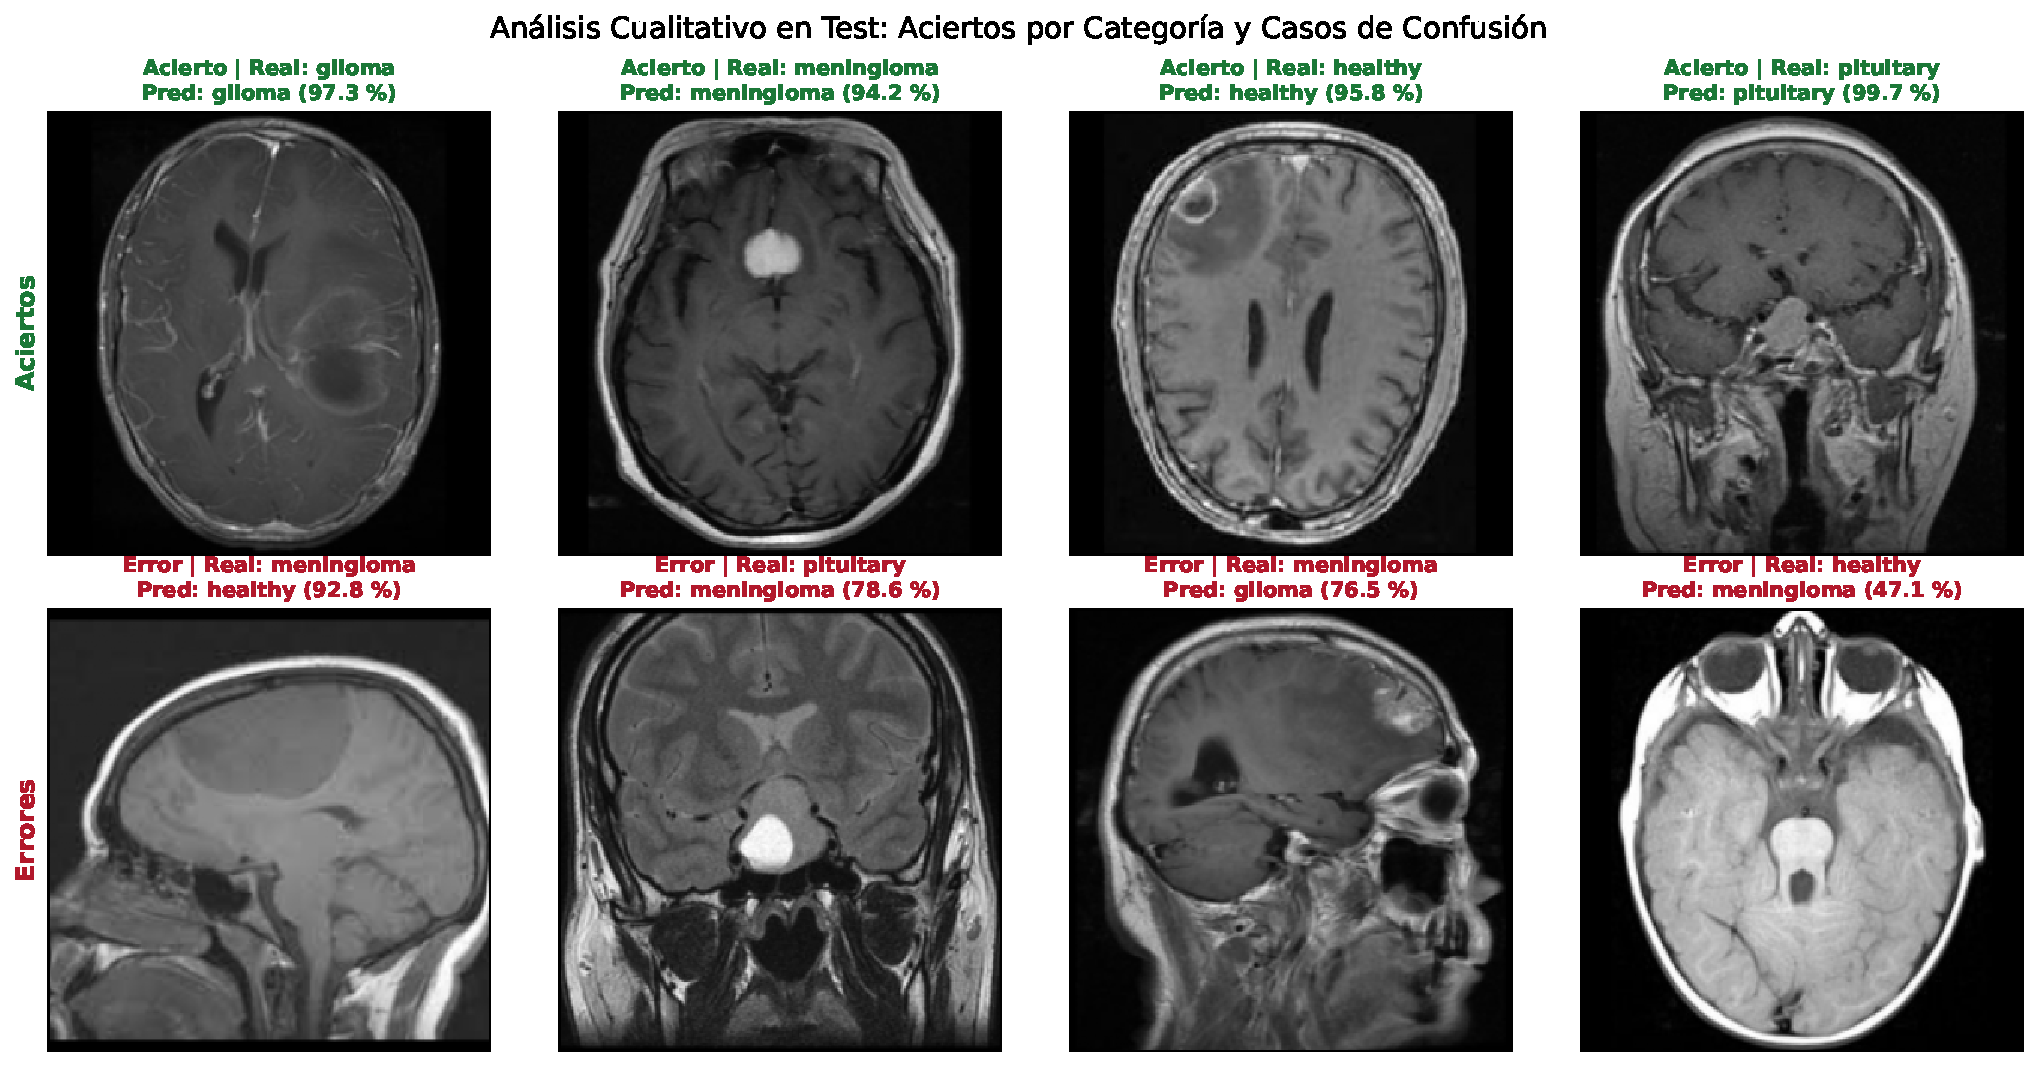
\includegraphics[width=0.98\linewidth]{figs/qualitative_predictions.pdf}
    \caption{Inspección cualitativa en \texttt{Test} ($n=990$): aciertos por clase (arriba) y errores de clasificación (abajo) con etiqueta real, predicción y confianza \texttt{softmax}.}
    \label{fig:qualitative}
\end{figure}

%%%%%%%%%%%%%%%%%%%%%%%%%%%%%%%%%%%%%%%%%%%%%%%%%%%%%%%%%%%%%%%%%%%%%%%%%%%%%%%%
\section{Discusión}

Los resultados obtenidos se explican a partir de tres mecanismos teóricos y experimentales:
\begin{itemize}
    \item \textbf{Capacidad representacional y campo receptivo:} Distinguir un \textit{glioma} infiltrativo de un \textit{meningioma} extraaxial circunscrito exige integrar bordes locales y contexto global. Apilar dos convoluciones $3\times 3$ por bloque (\texttt{DoubleConvMRICNN}) produce un campo receptivo efectivo de $5\times 5$ con doble no-linealidad antes de cada \texttt{MaxPool2d} \cite{c4}, mientras que concatenar \texttt{AdaptiveAvgPool2d} y \texttt{AdaptiveMaxPool2d} conserva tanto la activación máxima focal del tumor como la intensidad promedio del corte. Esto eleva el F1 de \textit{meningioma} de $59.77\,\%$ (\texttt{BaselineCNN} base en el subconjunto) a $92.31\,\%$ en exploración y hasta $97.38\,\%$ en \texttt{Test}, mientras que \textit{pituitary} ($99.62\,\%$), \textit{healthy} ($99.03\,\%$) y \textit{glioma} ($98.97\,\%$) superan el $98.9\,\%$.
    \item \textbf{Estabilidad del gradiente y calibración:} El uso conjunto de \texttt{CosineAnnealingLR}, suavizado de etiquetas ($\varepsilon=0.05$) \cite{c5} y recorte de gradiente reduce la varianza de \texttt{BatchNorm2d} en validación y evita sobreconfianza en los $12$ cortes ambiguos de \textit{meningioma} (confianzas medias de $44.9\,\%\text{--}78.6\,\%$).
    \item \textbf{Mitigación de \textit{data leakage} y \textit{shortcut learning}:} La eliminación de $426$ duplicados MD5, el recorte \texttt{CropToContent} y el desenfoque gaussiano aseguran que el modelo clasifique \textit{healthy} por su regularidad parenquimatosa y no por artefactos de borde o resolución \cite{c3}.
\end{itemize}

Como limitaciones del conjunto público destacan la ausencia de identificadores DICOM por paciente (cortes contiguos de un mismo estudio volumétrico podrían coexistir entre particiones pese a eliminar duplicados exactos) y la mezcla no anotada de planos y secuencias (T1c, T2, FLAIR). Como trabajo futuro se propone aplicar mapas de atribución visual (\textit{Grad-CAM}) sobre los $12$ casos de confusión de \textit{meningioma} y validar el modelo con partición agrupada por paciente.

%%%%%%%%%%%%%%%%%%%%%%%%%%%%%%%%%%%%%%%%%%%%%%%%%%%%%%%%%%%%%%%%%%%%%%%%%%%%%%%%
\begin{thebibliography}{99}

\bibitem{c1} D. N. Louis \textit{et al.}, ``The 2021 WHO classification of tumors of the central nervous system: a summary,'' \textit{Neuro-Oncology}, vol. 23, no. 8, pp. 1231--1251, 2021.

\bibitem{c2} S. Deepak and P. M. Ameer, ``Brain tumor classification using deep CNN features via transfer learning,'' \textit{Computers in Biology and Medicine}, vol. 111, p. 103345, 2019.

\bibitem{c3} R. Geirhos \textit{et al.}, ``Shortcut learning in deep neural networks,'' \textit{Nature Machine Intelligence}, vol. 2, no. 11, pp. 665--673, 2020.

\bibitem{c4} K. Simonyan and A. Zisserman, ``Very deep convolutional networks for large-scale image recognition,'' in \textit{Proc. Int. Conf. Learn. Represent. (ICLR)}, 2015, pp. 1--14.

\bibitem{c5} C. Szegedy \textit{et al.}, ``Rethinking the Inception architecture for computer vision,'' in \textit{Proc. IEEE Conf. Comput. Vis. Pattern Recognit. (CVPR)}, 2016, pp. 2818--2826.

\end{thebibliography}

\end{document}
